\documentclass[11pt, a4paper]{article}

% --- Packages ---
\usepackage[margin=2.5cm]{geometry}
\usepackage{setspace}
\usepackage{graphicx}
\usepackage{booktabs}
\usepackage{hyperref}
\usepackage[numbers, square]{natbib}
\usepackage{amsmath}
\usepackage{caption}
\usepackage{subcaption}
\usepackage{float}
\usepackage{microtype}
\usepackage[T1]{fontenc}
\usepackage[utf8]{inputenc}

% --- Single spacing as required ---
\singlespacing

% --- Figure path ---
\graphicspath{{../results/figures/}}

% --- Hyperlink styling ---
\hypersetup{
    colorlinks=true,
    linkcolor=blue,
    citecolor=blue,
    urlcolor=blue
}

% =========================================================
\begin{document}
% =========================================================

% --- Title ---
\begin{titlepage}
    \centering
    \vspace*{2cm}
    
    {\LARGE\bfseries Spatially Resolved Transcriptomics of the Small 
    Intestinal Villus and Its Microbiome Sensitivity\par}
    
    \vspace{1cm}
    {\large Replication and Extension of Mayassi et al. 2024\par}
    
    \vspace{2cm}
    {\large Wojciech Moryl\par}
    
    \vspace{0.5cm}
    {\large Modeling of Complex Biological Systems\par}
    
    \vspace{0.5cm}
    {\large \today\par}
    
    \vspace{3cm}
    \begin{abstract}
    The small intestinal epithelium is organized along two spatial axes: 
    a proximal-to-distal axis spanning duodenum, jejunum, and ileum, and 
    a vertical crypt-to-villus axis along which stem cells differentiate 
    into mature absorptive enterocytes. While Mayassi et al. 2024 
    comprehensively characterized regional transcriptional identity across 
    the gut using Visium spatial transcriptomics, their analysis focused 
    primarily on the colon, leaving the small intestinal villus layer 
    architecture largely uncharacterized. Here I replicate their spatial 
    framework and extend it by asking two questions: whether the 
    crypt-to-villus transcriptional gradient is conserved across SI 
    segments, and whether the microbiome differentially affects gene 
    expression along this axis. I find that a large conserved core 
    program exists across all four SI segments — 646 crypt markers and 
    2,381 villus tip markers shared across duodenum, jejunum1, jejunum2, 
    and ileum — overlaid with region-specific gene expression that 
    increases toward the villus tip. GO enrichment confirms the biological 
    validity of these layers: conserved crypt markers are enriched for 
    cell cycle and DNA replication terms, while conserved tip markers 
    reflect the secretory pathway and vesicle transport. Comparing 
    germ-free and specific-pathogen-free mice, I find that the microbiome 
    asymmetrically affects the crypt-to-villus axis: the bottom villous SI 
    is most transcriptionally promoted by microbiome presence, while the 
    villus tip shows unexpected upregulation of mRNA processing, 
    translation, and protein catabolism in germ-free mice, suggesting 
    the microbiome induces transcriptional restraint at the most 
    exposed epithelial surface.
    \end{abstract}
\end{titlepage}

% =========================================================
\section{Introduction}
% =========================================================

The mammalian small intestine is responsible for the absorption of 
virtually all dietary nutrients, a function carried out by a 
specialized epithelium organized into villi. Each villus is a dynamic 
structure maintained by a continuous process of cell renewal: 
intestinal stem cells at the base of crypts ivide and give rise to 
transit-amplifying progenitors, which migrate upward along the villus, 
differentiating into mature absorptive enterocytes as they go, and 
eventually shedding from the villus tip into the gut lumen 
\cite{kai2021intestinal}. This crypt-to-villus 
axis represents one of the most visible differentiation gradients in 
mammalian biology, with cells transitioning from rapidly dividing 
stem cells to post-mitotic, functionally specialized absorptive cells 
over a period of just three to five days \cite{barrett2018mapping}.

The three major segments of the small intestine — duodenum, jejunum, 
and ileum — each perform distinct physiological roles. The duodenum 
receives preprocessed food from the stomach and neutralizes gastric acid, 
while absorbing iron, calcium and fat-soluble vitamins 
(A, D, E, K). The jejunum is the primary site of monosaccharides, 
amino acid, and lipid absorption. The ileum specializes in bile acid 
reabsorption, water-soluble vitamins (B12, C) uptake, and 
contains the highest density of immune cells \cite{santaolalla2011innate}. 
These regional differences are reflected in distinct transcriptional 
programs, though the extent to which the crypt-to-villus axis itself 
differs across segments has not been well characterized.

Mayassi et al. 2024 performed a landmark spatial transcriptomics 
study of the mouse gut using Visium technology, generating a 
comprehensive atlas of ~120,000 tissue spots spanning the entire 
gastrointestinal tract \cite{mayassi2024}. Their key finding was 
that regional transcriptional identity is remarkably robust to 
microbiome perturbation — germ-free and conventionally housed mice 
maintain similar spatial gene expression patterns across the gut. 
They further identified a microbiota-driven transcriptional region 
in the mid-colon. However, their analysis focused predominantly on 
colonic regionalization, since that is where they found the most 
distinctive patterns, and the spatial architecture of the small 
intestinal villus — particularly the crypt-to-villus axis — was 
not deeply characterized.

In this work, I replicate parts of the spatial framework established 
by Mayassi et al. and extend the analysis to the small intestinal 
villus layer axis. I address two questions: (1) Is the 
crypt-to-villus transcriptional gradient conserved across SI 
segments, or does each segment have a unique villus program? 
(2) Does microbiome presence differentially affect gene expression 
along the crypt-to-villus axis? I hypothesized that a conserved 
core villus program exists across segments, and that the villus 
tip — directly exposed to luminal bacteria — would be more 
microbiome-sensitive than the protected crypt.

% =========================================================
\section{Methods and Materials}
% =========================================================

\subsection{Data}

Visium spatial transcriptomics data were obtained from the Broad 
Single Cell Portal (accession SCP2762), corresponding to the 
microbiome experiment described in Mayassi et al. 2024. The dataset 
comprises 120,021 Visium spots from mouse small intestine and colon, 
spanning four small intestinal regions (Duodenum, Jejunum1, Jejunum2, 
Ileum) and colon, across three microbiome conditions: specific 
pathogen-free (SPF), germ-free (GF), and fecal microbiota transplant 
(FMT). Each spot captures RNA from approximately 5-15 cells at a 
55 $\mu$m diameter resolution. Spot-level metadata including tissue 
region, villus layer annotation (ylayer), and microbiome condition 
were provided by the authors. The ylayer annotation assigns each 
spot to one of four categories: Crypt SI, Bottom villous SI, 
Top villous SI, or Muscle SI.

\subsection{Preprocessing}

Raw count matrices were loaded using \texttt{scipy.io} and assembled 
into AnnData objects using Scanpy v1.12.1 \cite{wolf2018scanpy}. 
Quality control metrics were calculated using 
\texttt{sc.pp.\allowbreak calculate\_qc\_\allowbreak metrics}, flagging mitochondrial genes 
by the \texttt{mt-} prefix. Spots with fewer than 500 counts, fewer 
than 200 detected genes, or more than 20\% mitochondrial counts were 
removed as likely damaged tissue (standard tresholds), resulting in 
119,892 spots retained for analysis (the data was already 
prepocessed by the authors). Highly variable genes were selected 
on raw counts using the seurat\_v3 method (n=3,000). Raw counts 
were stored prior to normalization. Spots were normalized to 
10,000 counts per spot and log1p (to avoid log(0)) transformed. 
Principal component analysis was performed on the 3,000 highly 
variable genes (\texttt{zero\_center=False} to preserve sparsity). 
A k-nearest neighbor graph was computed (k=15, n\_pcs=30) and UMAP 
embedding was computed for visualization.

\subsection{Leiden Clustering}

Leiden unsupervised clustering was performed on the data using several
resolution parameters (0.02, 0.05, 0.1, 0.25 and 0.5) to check if 
whether indepentent clustering would recapture the known (and annotated
by the authors) regional and layer structure of the data. The
clustering at resolution=0.5 yielded in 27 clusters that are largely
region-pure (Figure heatmap), but each region was split into multiple
subclusters corresponding to "petals" substructure of the UMAP, not 
to the known villus layers. At lowest resolution (0.02) the clustering
produced 4 clusters - which is the same number as the number of 
annotated regions - but the clusters are not pure and the two jejunum 
regions mix the most. This could confirm that both proximal-distal axis 
and, even more so, the crypt-villus tip axis form somewhat continuous 
gradient and the regions located next to each other cannot be easily 
separated by the unsupervised clutstering. For this reason, I decided 
to use the pre-existing authors' anntotations (tissue region and ylayer)
direclty for the DEG analysis.

\subsection{Differential Expression Analysis}

Differential expression analysis was performed using the Wilcoxon 
rank-sum test implemented in Scanpy 
(\texttt{sc.tl.rank\_genes\_groups}). This non-parametric test
was chosen because gene expression data in spatial transcriptomics
is highly skewed and that violates the normality assumption of 
parametric tests. For regional marker identification, each SI 
region was compared against all other regions (one-vs-rest). 
For villus layer marker identification, analysis was restricted 
to epithelial spots (Crypt SI, Bottom villous SI, Top villous SI). 
Muscle SI was excluded since it does not represent an epithelial
layer and so would only be confouning for the analysis. Significant 
DEGs were defined by adjusted p-value $<$ 0.05 and $|\log_2 FC|$ 
$>$ 0.5. For the microbiome comparison (SPF vs GF), the larger 
condition was downsampled to match the smaller condition within 
each region $\times$ layer combination prior to analysis 
(random seed = 42) to ensure equal statistical power. A minimum 
log2 fold change threshold of 0.25 was applied for directional 
analysis. The lower log2 fold change threshold for the microbiome
comparison was chosen to capture the expected subtler differences.

\subsection{Conservation Analysis}

To assess conservation of villus layer markers across SI segments, 
DEG analysis was performed independently within each of the four 
SI regions for each villus layer. Genes identified as significant 
markers in all four regions were classified as conserved core markers. 
Genes significant in only one region were classified as 
region-specific markers.

\subsection{Gene Ontology Enrichment}

GO enrichment analysis was performed using gseapy v1.2.1 
\cite{fang2023enrichr} via the Enrichr API, querying the 
GO Biological Process 2023 database. Mouse gene symbols were 
used directly. Significant GO terms were defined by adjusted 
p-value $<$ 0.05. Mitochondrial genes were excluded from 
visualization of marker gene expression heatmaps, as they 
reflect general cellular energy demand rather than 
layer-specific functional identity.

\subsection{Reproducibility}

All analyses were performed in Python 3.11 within a conda 
environment. The complete workflow is defined in a Snakefile 
and executed via Snakemake v9.22.0 using papermill v2.7.0 
for notebook execution. Code and notebooks are available at 
\url{https://github.com/Fair0n/gut-transcriptomics-project}.

% =========================================================
\section{Results}
% =========================================================

\subsection{Replication of Spatial Framework}

I successfully replicated the spatial transcriptomics framework 
established by Mayassi et al. 2024. The unrolled gut visualization 
(Figure \ref{fig:unrolled}) reproduces the tissue architecture 
described in the original paper, with the proximal-to-distal gut 
axis represented on the X axis and the crypt-to-villus axis on 
the Y axis. The villus layer annotations (Crypt SI, Bottom villous 
SI, Top villous SI, Muscle SI) are clearly visible as distinct 
horizontal bands within each regional section.

\begin{figure}[H]
    \centering
    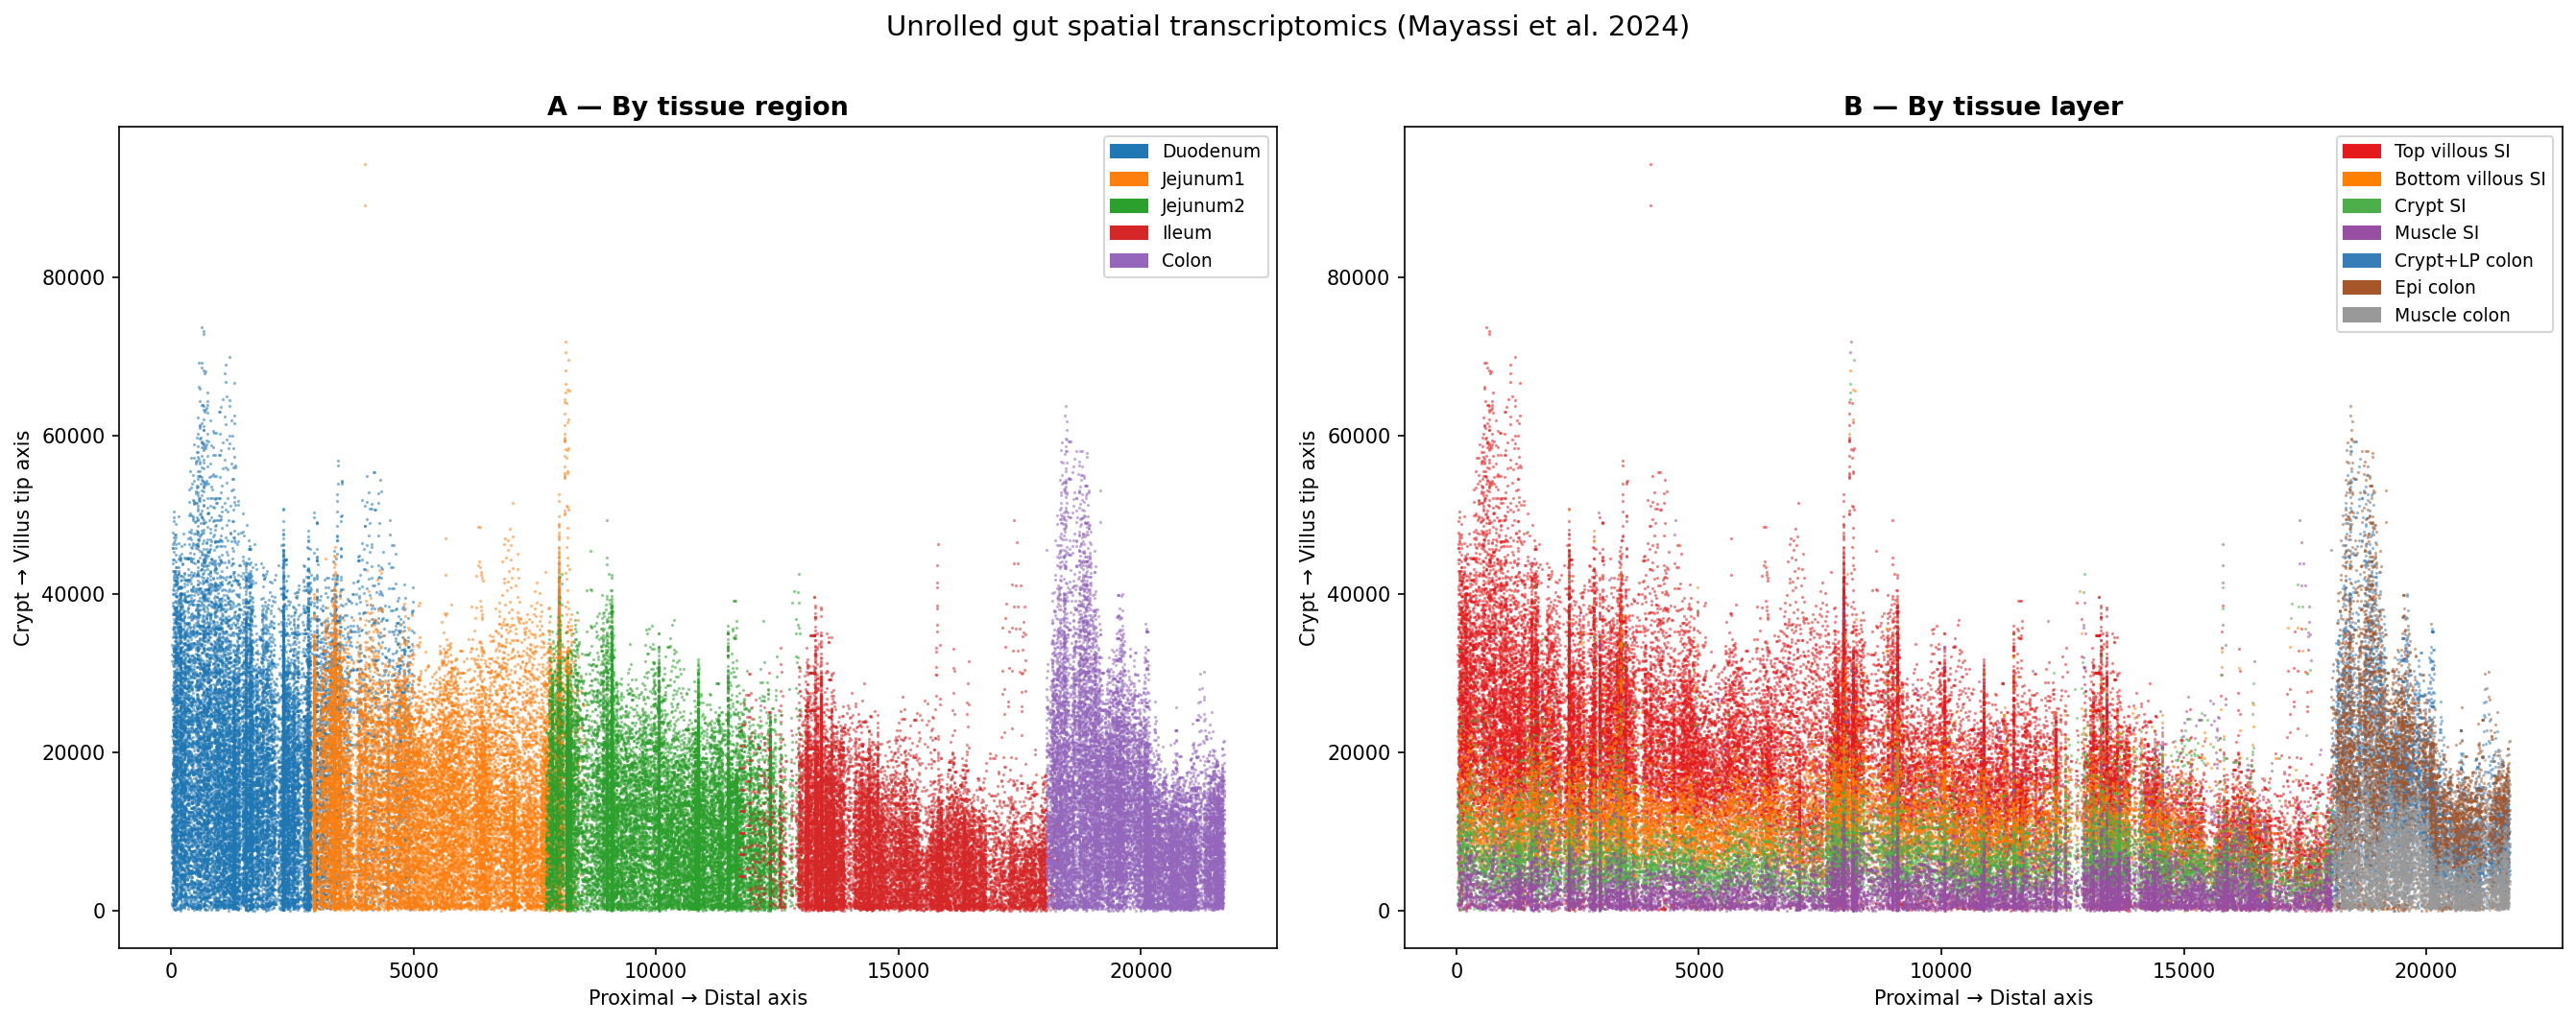
\includegraphics[width=\textwidth]{01_unrolled_gut_overview.png}
    \caption{Unrolled gut spatial transcriptomics overview. Left: 
    spots colored by tissue region. Right: spots colored by villus 
    layer annotation. The X axis represents the proximal-to-distal 
    gut axis; the Y axis represents the crypt-to-villus tip axis.}
    \label{fig:unrolled}
\end{figure}

UMAP embedding of all 119,892 spots (Figure \ref{fig:umap}) shows 
clear separation between gut regions, with small intestine and colon 
forming distinct clusters. SPF and GF spots intermix 
throughout the UMAP, confirming the paper's core finding that 
regional transcriptional identity is robust to microbiome presence.

\begin{figure}[H]
    \centering
    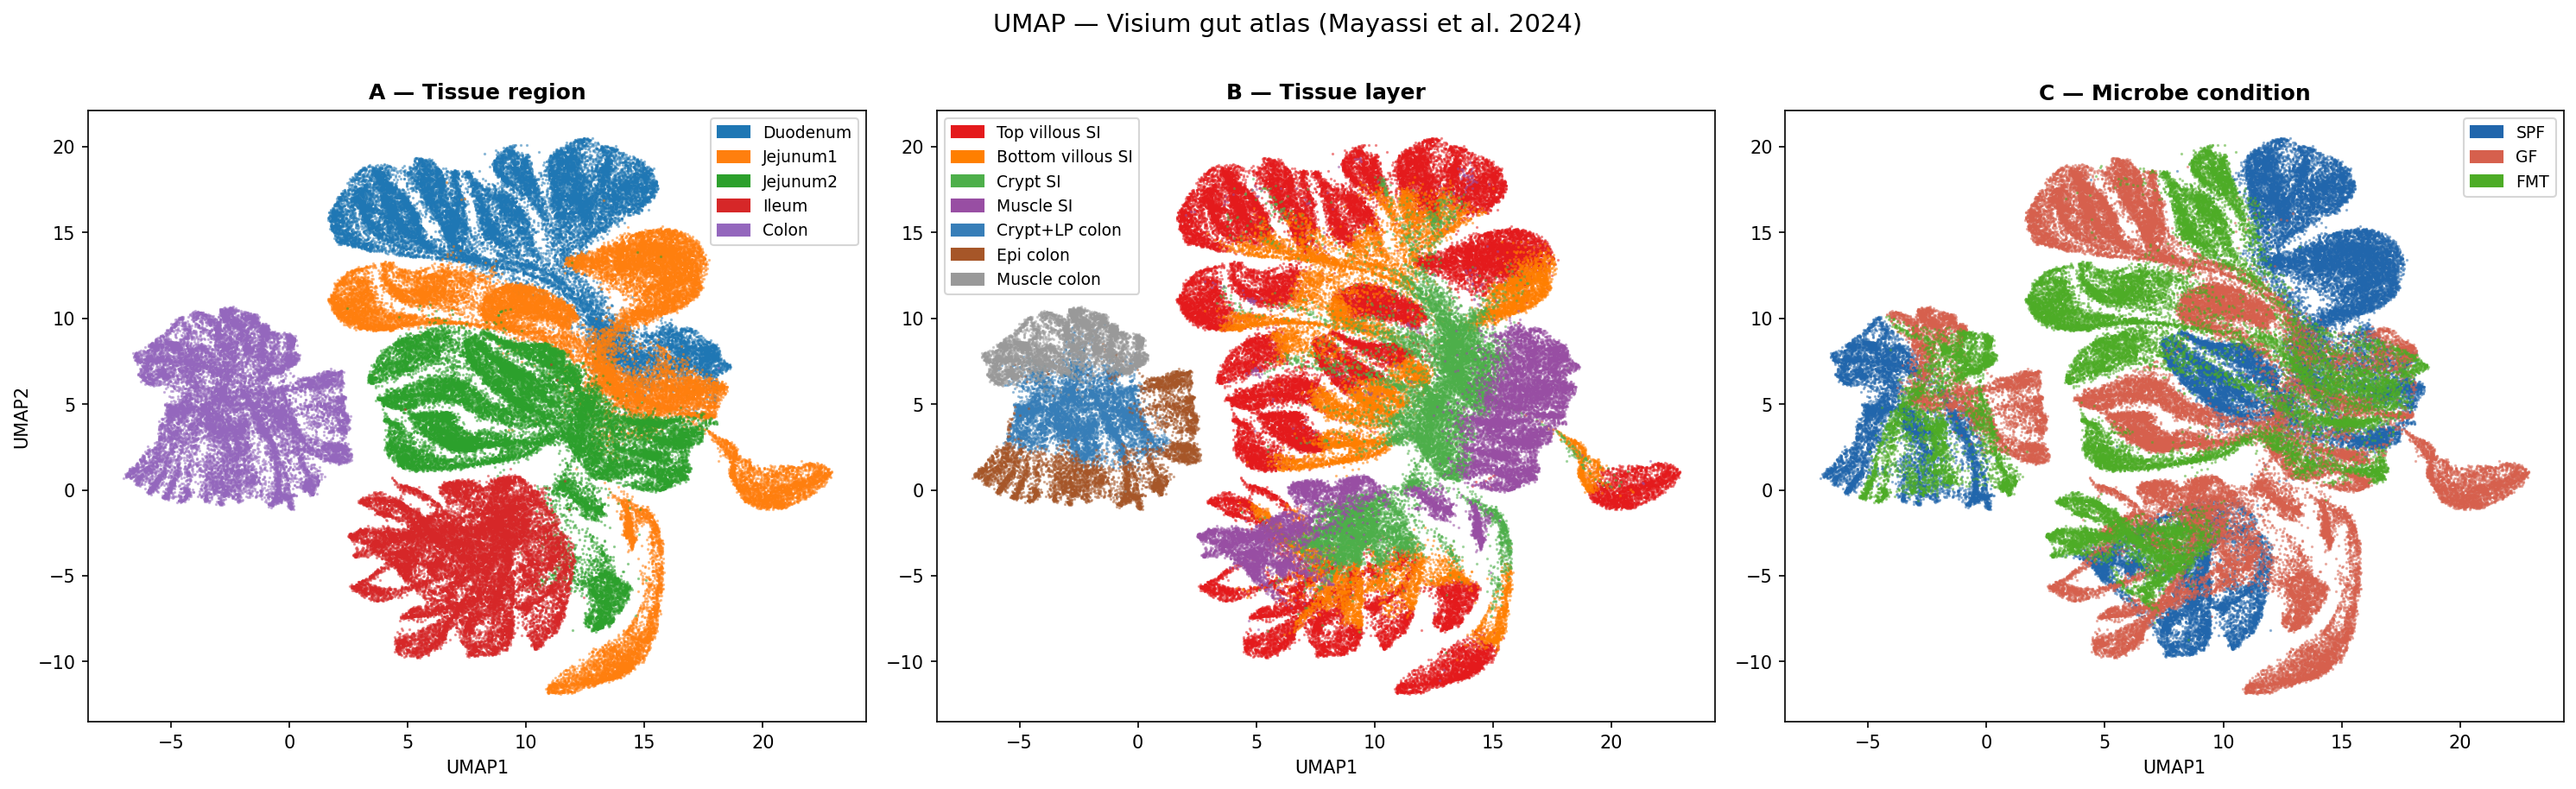
\includegraphics[width=\textwidth]{02_umap_overview.png}
    \caption{UMAP of all Visium spots colored by tissue region (A), 
    villus layer (B), and microbiome condition (C). SPF and GF spots 
    intermix throughout, confirming transcriptional robustness to 
    microbiome perturbation.}
    \label{fig:umap}
\end{figure}

\subsection{Small Intestinal Regional Identity}

Restricting analysis to small intestine spots and recomputing the 
UMAP provides a more detailed view of SI-specific transcriptional structure
(Figure \ref{fig:si_umap}). All four SI regions form distinct clusters
with an internal "flower" structure reflecting the villus layer 
organization within each segment.

\begin{figure}[H]
    \centering
    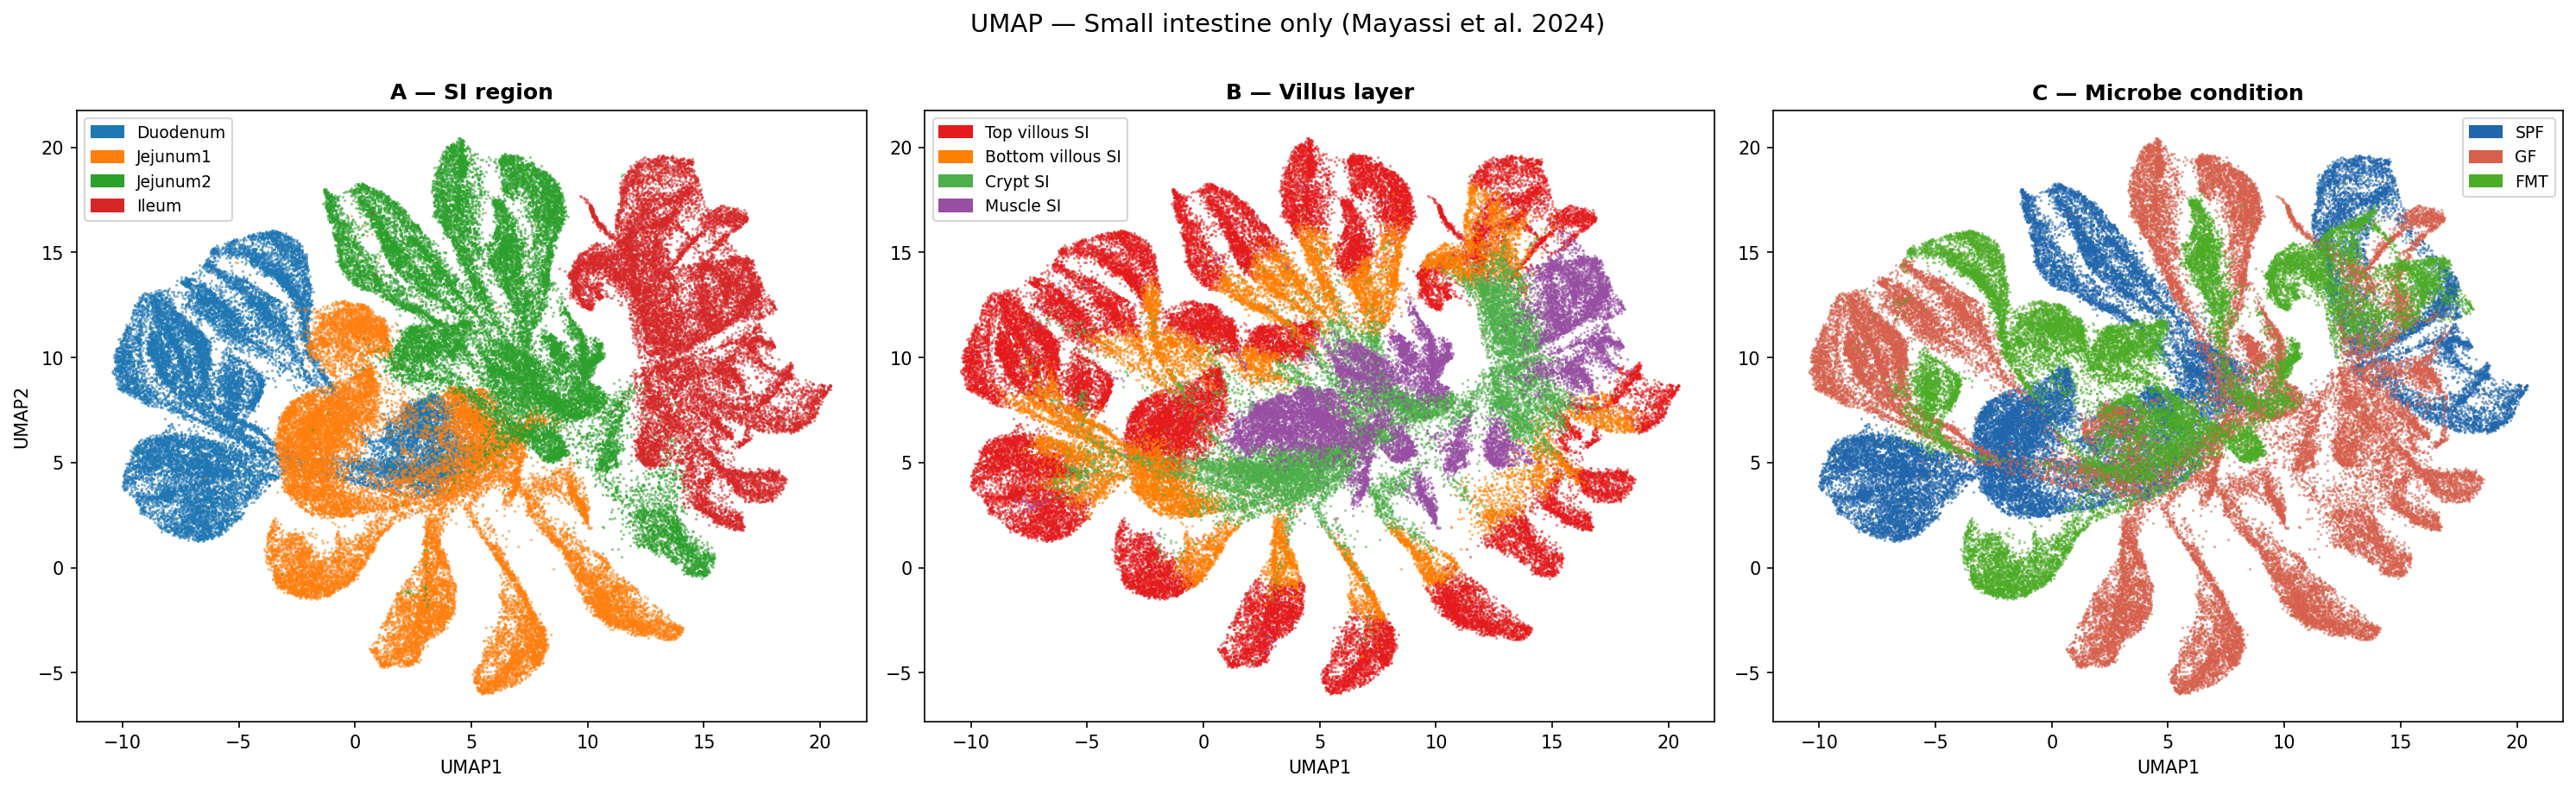
\includegraphics[width=\textwidth]{03_si_umap.png}
    \caption{UMAP of small intestine spots only, colored by region 
    (A), villus layer (B), and microbiome condition (C). Each region 
    forms a distinct cluster with internal villus layer structure.}
    \label{fig:si_umap}
\end{figure}

Differential expression analysis identified 6,406 significant 
regional marker genes across all four SI segments. The ileum showed 
the most unique transcriptional identity (2,801 DEGs), followed by 
duodenum (1,929), jejunum1 (1,075), and jejunum2 (601). Top marker 
genes for each region are biologically validated: duodenum markers 
include \textit{Reg1} and \textit{S100g}, jejunum markers include 
\textit{Fabp1} and \textit{Apoa4} (fatty acid and lipoprotein 
absorption), and ileum markers include \textit{Fabp6} (bile acid 
binding) and \textit{Tmigd1} (Figure \ref{fig:dotplot_region}).

\begin{figure}[H]
    \centering
    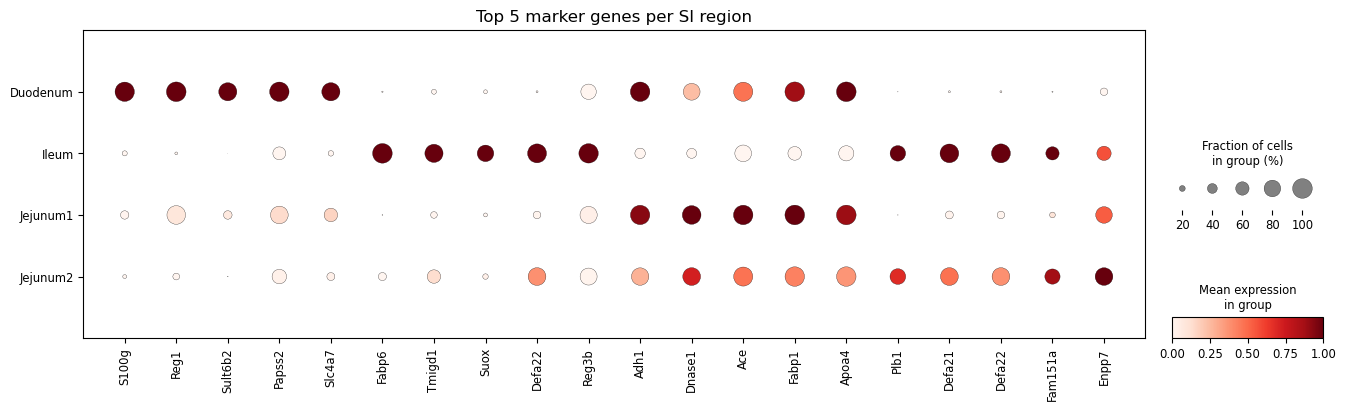
\includegraphics[width=\textwidth]{dotplot_03_region_marker_dotplot.png}
    \caption{Dotplot of top 5 marker genes per SI region. Dot size 
    indicates the fraction of spots expressing the gene; color 
    indicates mean expression level (scaled 0-1 per gene).}
    \label{fig:dotplot_region}
\end{figure}

\subsection{Conservation of the Crypt-to-Villus Transcriptional Gradient}

To characterize the crypt-to-villus axis, I performed differential 
expression analysis between Crypt SI, Bottom villous SI, and Top 
villous SI spots, first across all SI regions combined and then 
independently within each region. Across all regions, 8,870 
significant layer DEGs were identified, with Top villous SI showing 
the most (4,313), followed by Bottom villous SI (3,245) and 
Crypt SI (1,312), which is not surprising given the increasing
functional specialization present toward the villus tip.

Crypt SI markers are dominated by proliferation and cell cycle genes, 
including \textit{Mki67} (canonical proliferation marker), 
\textit{Olfm4} (intestinal stem cell marker), and \textit{Stmn1} 
(expressed in rapidly dividing progenitors), validating the 
biological accuracy of the layer annotations 
(Figure \ref{fig:dotplot_layer}).

\begin{figure}[H]
    \centering
    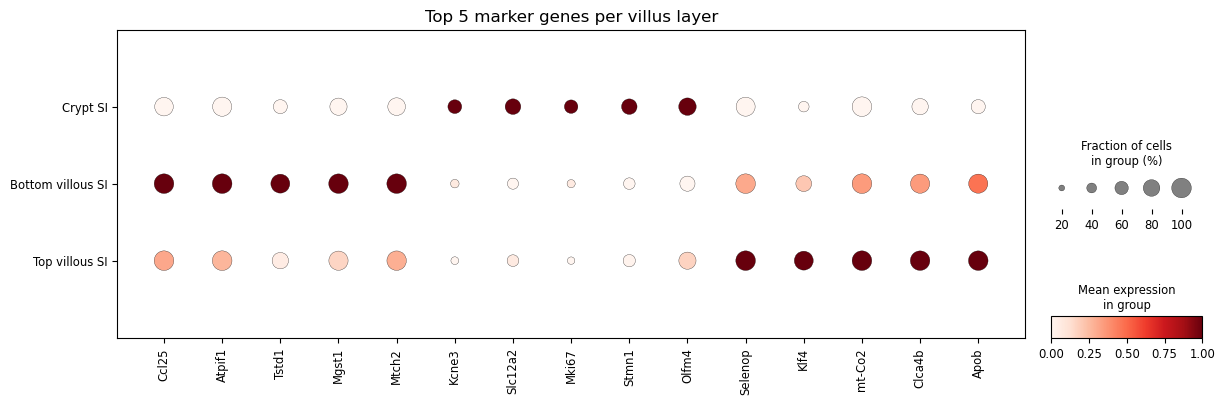
\includegraphics[width=\textwidth]{dotplot_03_layer_marker_dotplot.png}
    \caption{Dotplot of top 5 marker genes per villus layer. Layers 
    are ordered from crypt base (bottom) to villus tip (top), 
    reflecting the direction of cell migration. Key markers include 
    \textit{Mki67} and \textit{Olfm4} (Crypt SI) and \textit{Apob} 
    and \textit{Klf4} (Top villous SI).}
    \label{fig:dotplot_layer}
\end{figure}

Conservation analysis revealed that a large conserved core program 
is shared across all four SI segments for each villus layer 
(Figure \ref{fig:conservation}): 646 conserved crypt markers, 
2,224 conserved bottom villous markers, and 2,381 conserved top 
villous markers. The villus tip shows both the largest conserved 
core and the largest region-specific component, with the ileum 
contributing the most unique tip markers (975 region-specific genes).
This is most likely because the cells at the villus tip are the most 
specialized, and therefore they have both the highest number of markers
overall and the highest number of region-specific markers.

\begin{figure}[H]
    \centering
    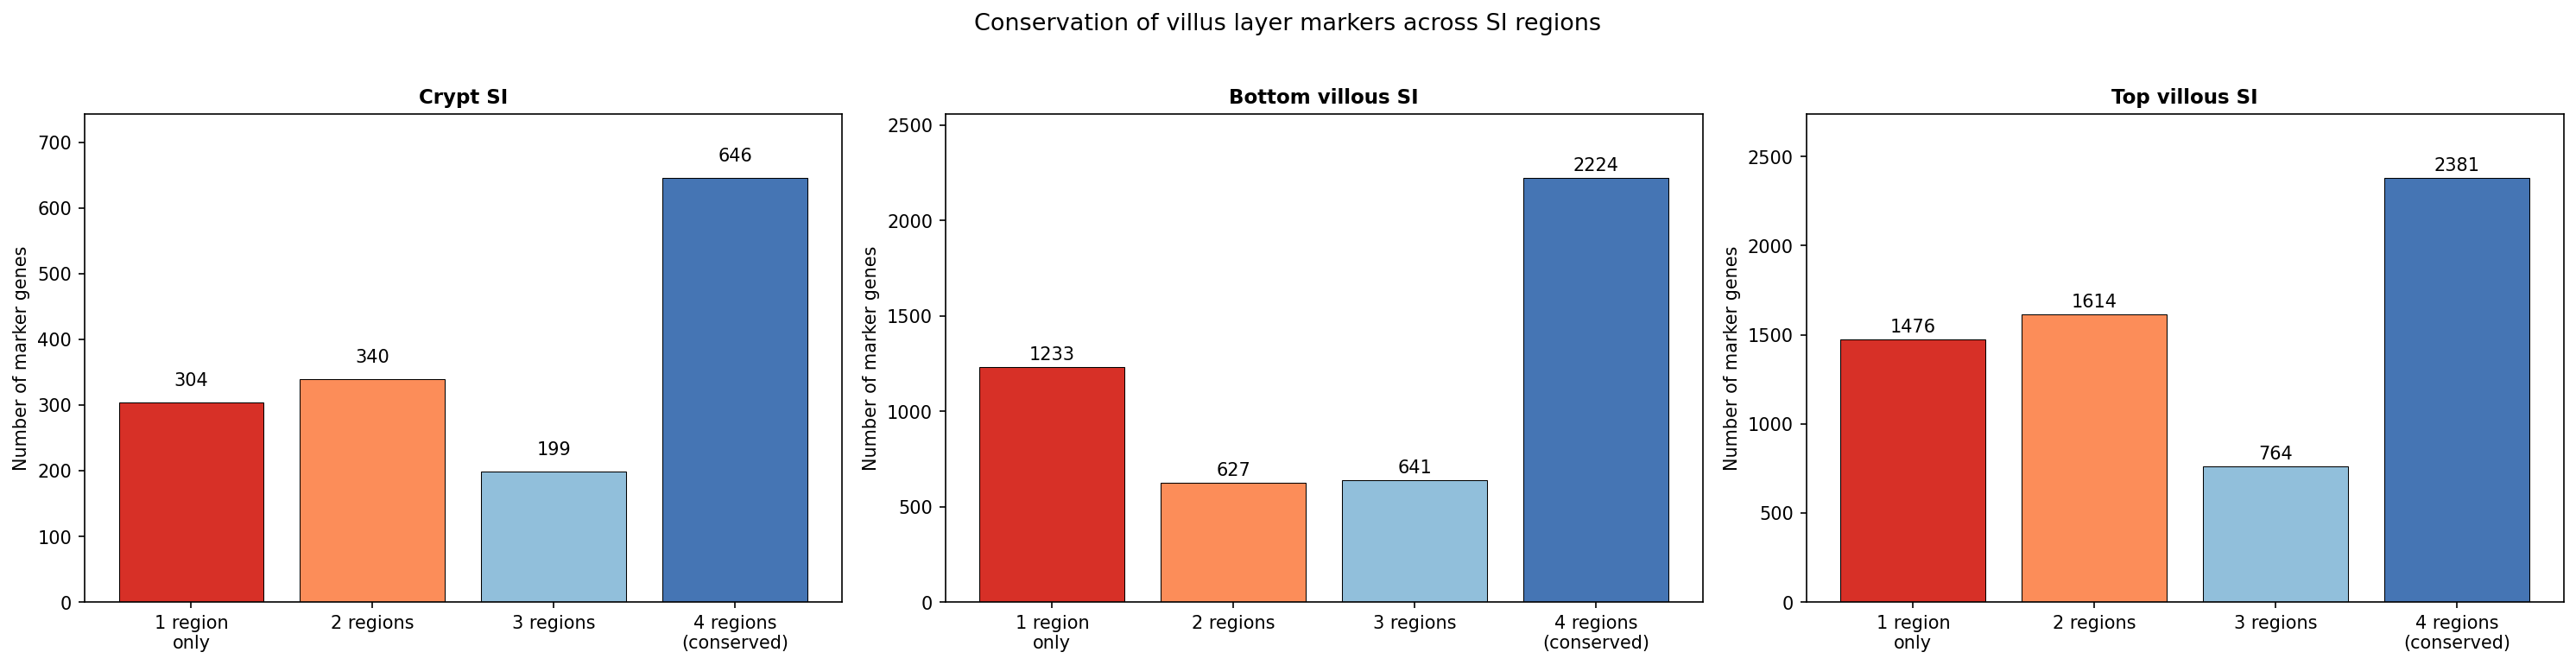
\includegraphics[width=\textwidth]{03_layer_marker_conservation.png}
    \caption{Conservation of villus layer markers across SI regions. 
    For each layer, marker genes are classified by how many regions 
    they appear in (1 = region-specific, 4 = conserved across all 
    segments). The blue bar represents the conserved core shared 
    by all four SI regions.}
    \label{fig:conservation}
\end{figure}

Expression of the top conserved villus tip markers (excluding 
mitochondrial genes) across all region-layer combinations confirms 
a gradient of increasing expression from crypt to villus tip 
(Figure \ref{fig:heatmap}). Key conserved tip markers include 
\textit{Apob} (apolipoprotein B, required for chylomicron assembly 
and fat absorption), \textit{Klf4} (transcription factor marking 
terminally differentiated enterocytes), \textit{Slc6a19} (neutral 
amino acid transporter), and MHC class I molecules \textit{H2-K1} 
and \textit{H2-D1}.

\begin{figure}[H]
    \centering
    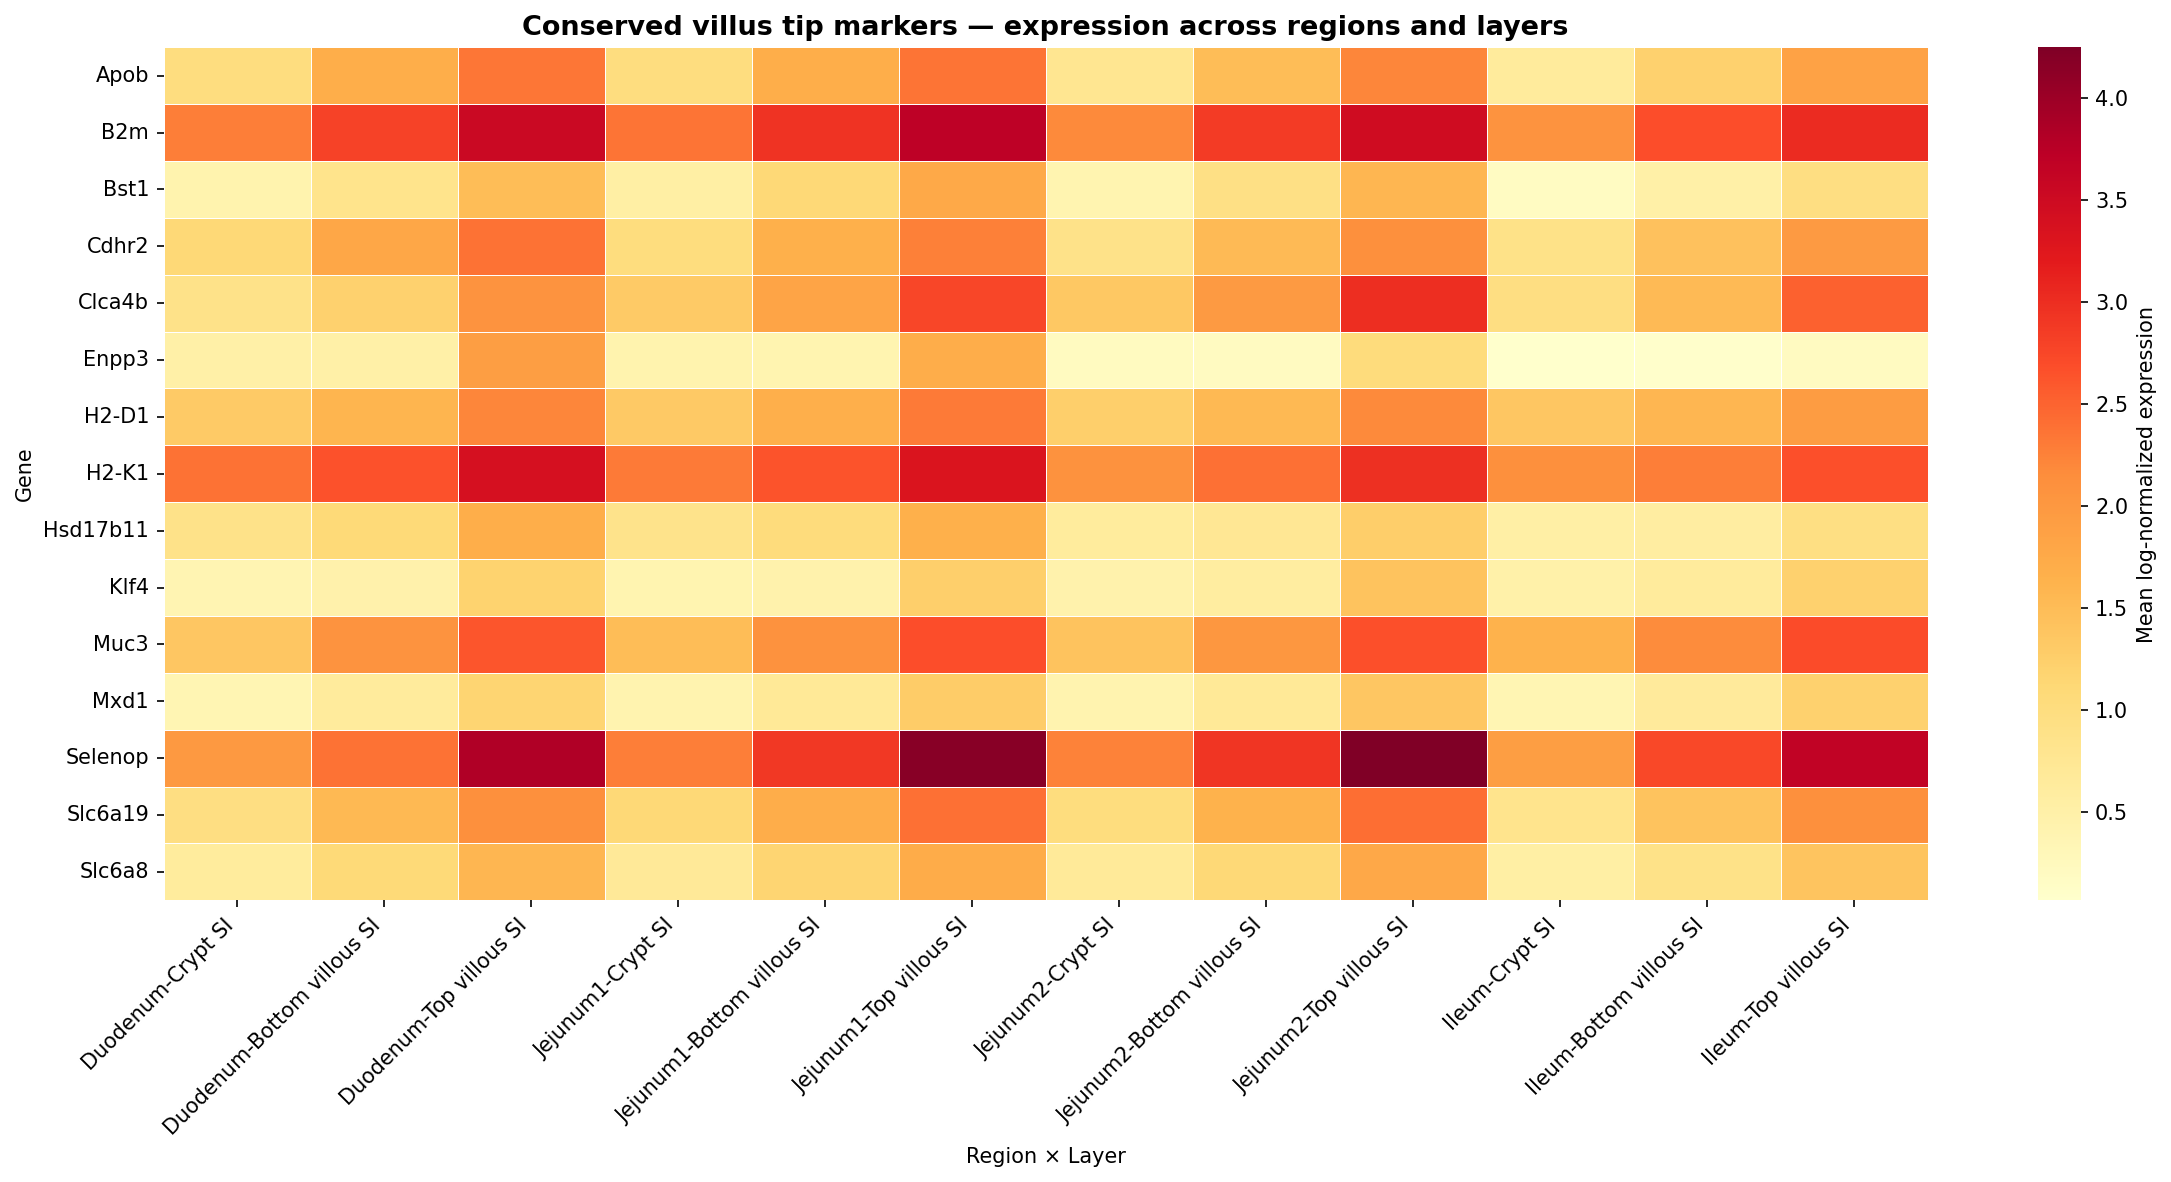
\includegraphics[width=\textwidth]{03_conserved_tip_markers_heatmap.png}
    \caption{Mean expression of top conserved villus tip markers 
    across all region-layer combinations. Columns are ordered 
    Crypt $\rightarrow$ Bottom villous $\rightarrow$ Top villous 
    within each region, reflecting the biological gradient. 
    Mitochondrial genes excluded for clarity.}
    \label{fig:heatmap}
\end{figure}

\subsection{Gene Ontology Enrichment of Villus Layer Markers}

GO enrichment of conserved layer markers confirms the biological 
identity of each layer (Figure \ref{fig:go}). Conserved Crypt SI 
markers are highly enriched for cell cycle and DNA replication terms 
(Mitotic Sister Chromatid Segregation, DNA Metabolic Process, 
Positive Regulation of Cell Cycle Process), consistent with the 
crypt's role as the proliferative compartment. Conserved Top 
villous SI markers are enriched for vesicle transport and secretory 
pathway terms (Golgi Vesicle Transport, ER-to-Golgi Transport, 
Vesicle-Mediated Transport), reflecting the continuous secretion 
of chylomicrons, mucus, and antimicrobial peptides by mature 
enterocytes at the villus tip.

\begin{figure}[H]
    \centering
    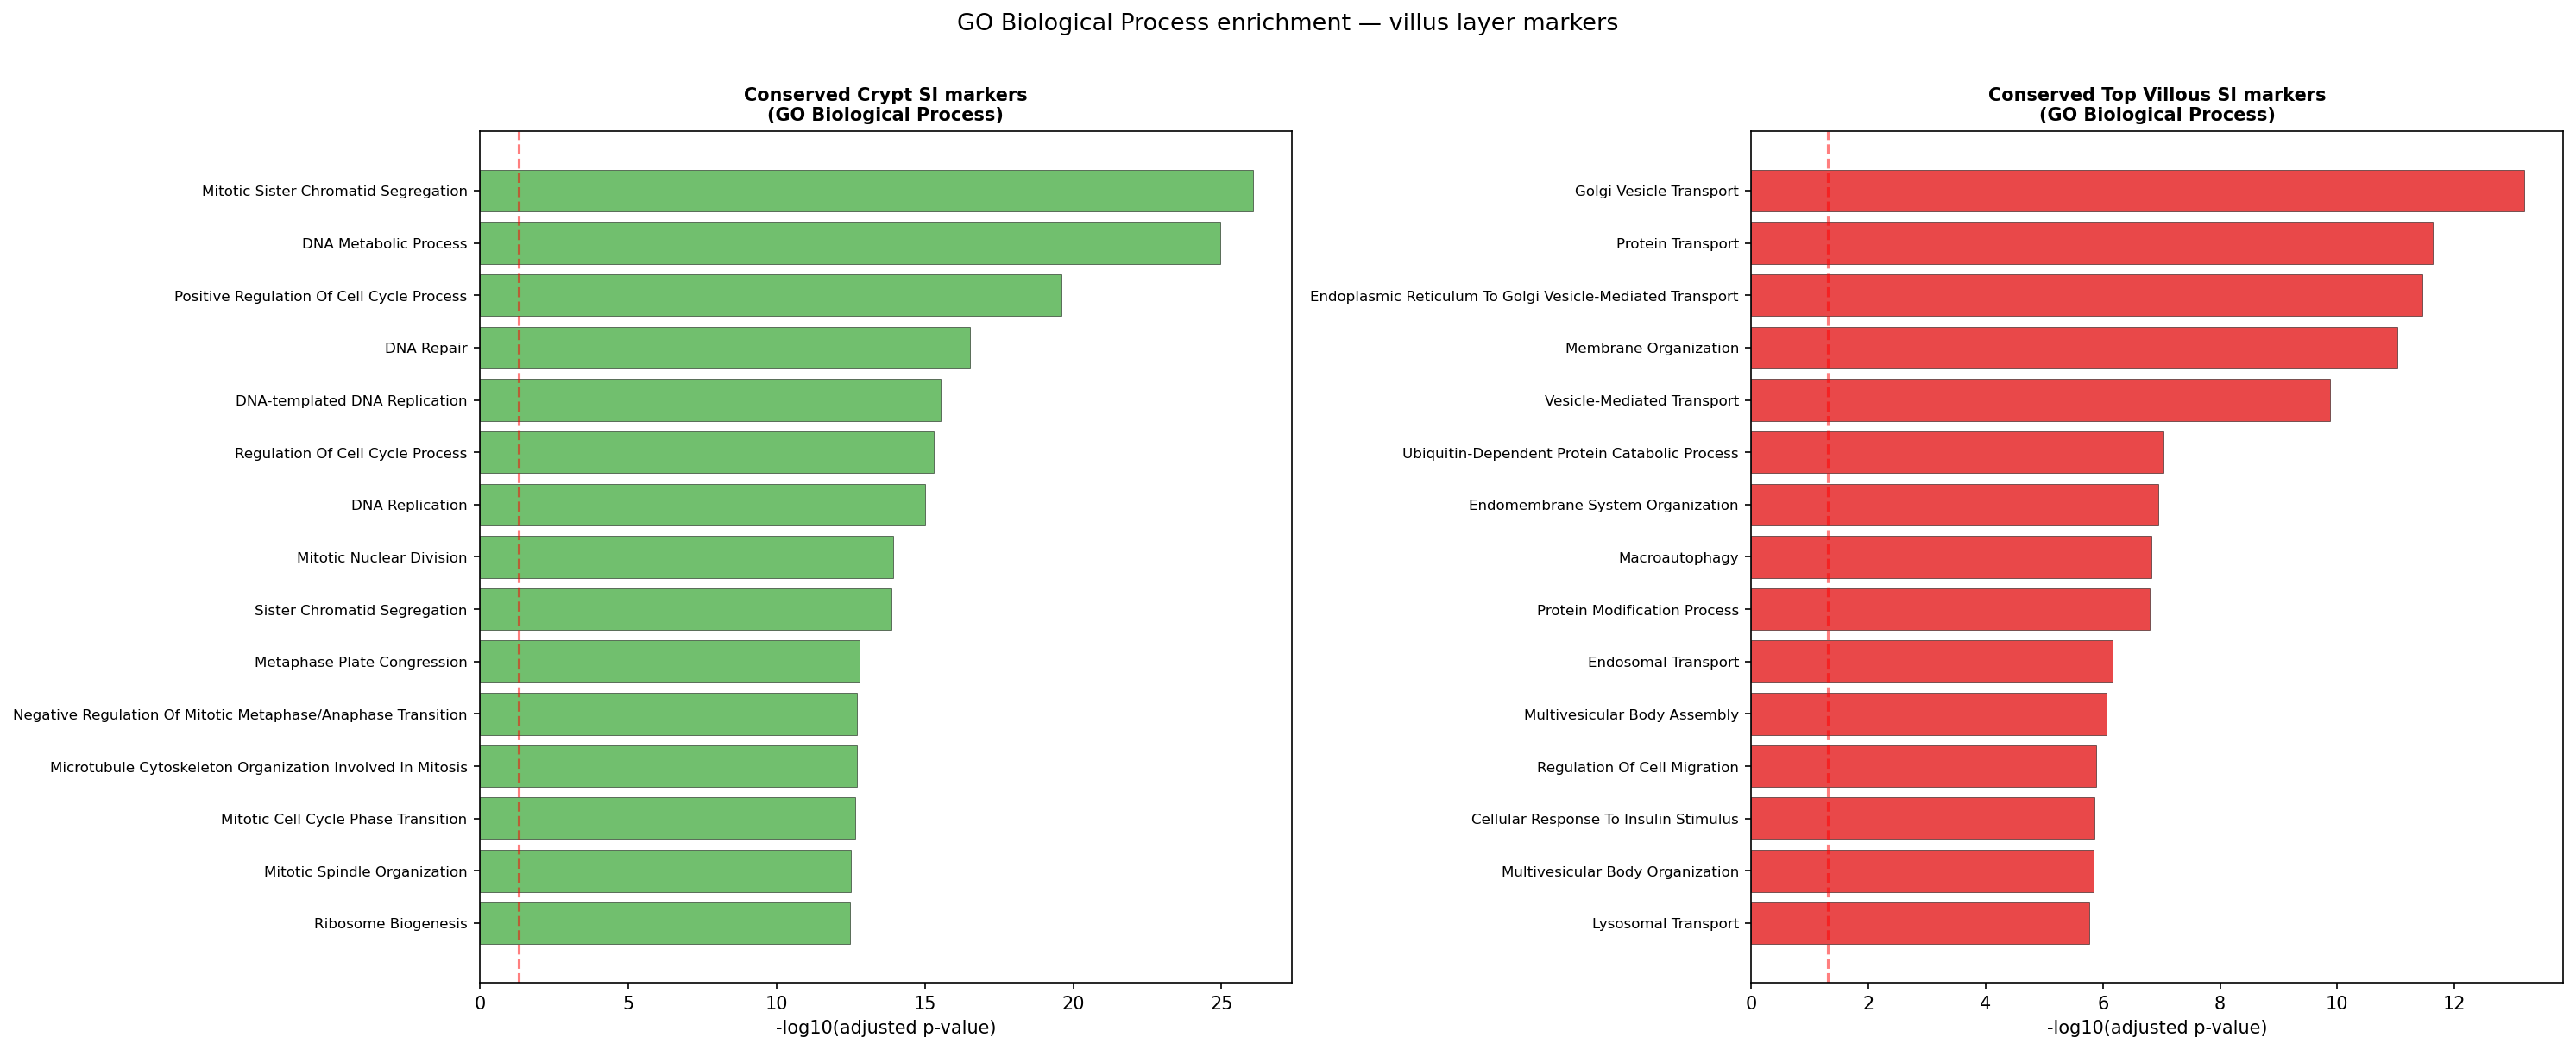
\includegraphics[width=\textwidth]{04_go_crypt_vs_top_villous.png}
    \caption{GO Biological Process enrichment for conserved Crypt SI 
    markers (green) and conserved Top villous SI markers (red). 
    Bars show $-\log_{10}$(adjusted p-value). Red dashed line marks 
    the p=0.05 significance threshold.}
    \label{fig:go}
\end{figure}

\subsection{Microbiome Differentially Affects the Crypt-to-Villus Axis}

To test whether the microbiome affects gene expression differently 
along the crypt-to-villus axis, I compared SPF and GF spots within 
each of the 12 region-layer combinations, downsampling to equal 
spot counts per condition to ensure fair comparison. The results 
reveal a striking asymmetry (Figure \ref{fig:microbiome}).

\begin{figure}[H]
    \centering
    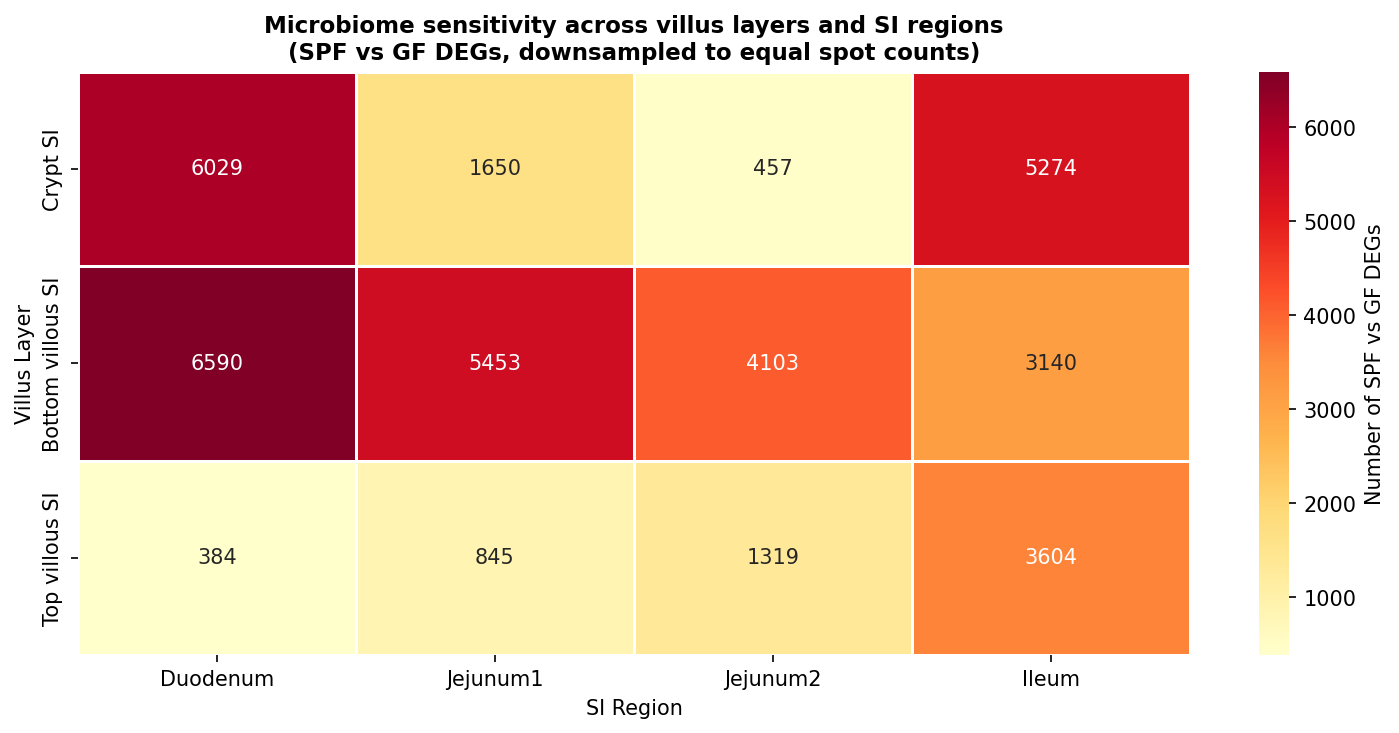
\includegraphics[width=\textwidth]{05_microbiome_sensitivity_heatmap.png}
    \caption{Number of SPF vs GF differentially expressed genes per 
    region-layer combination. Left: genes upregulated in SPF 
    (promoted by microbiome). Right: genes upregulated in GF 
    (suppressed by microbiome). Both conditions were downsampled 
    to equal spot counts prior to analysis.}
    \label{fig:microbiome}
\end{figure}

The Bottom villous SI is consistently the most microbiome-promoted 
layer across all SI regions (3,142-6,600 SPF-upregulated DEGs), 
suggesting the microbiome primarily influences the enterocyte 
maturation zone rather than stem cell identity or fully 
differentiated cells.

Contrary to my initial hypothesis, the Top villous SI shows 
the largest GF-upregulation rather than SPF-upregulation — 
thousands of genes are upregulated at the villus tip specifically 
in germ-free mice (6,431 in Duodenum, 6,147 in Jejunum1, 3,224 
in Jejunum2, 1,362 in Ileum). GO enrichment of these GF-upregulated 
top villous genes reveals enrichment for mRNA Processing, Gene 
Expression, RNA Splicing, Translation, and Protein Catabolism 
(Figure \ref{fig:go_tip}).

\begin{figure}[H]
    \centering
    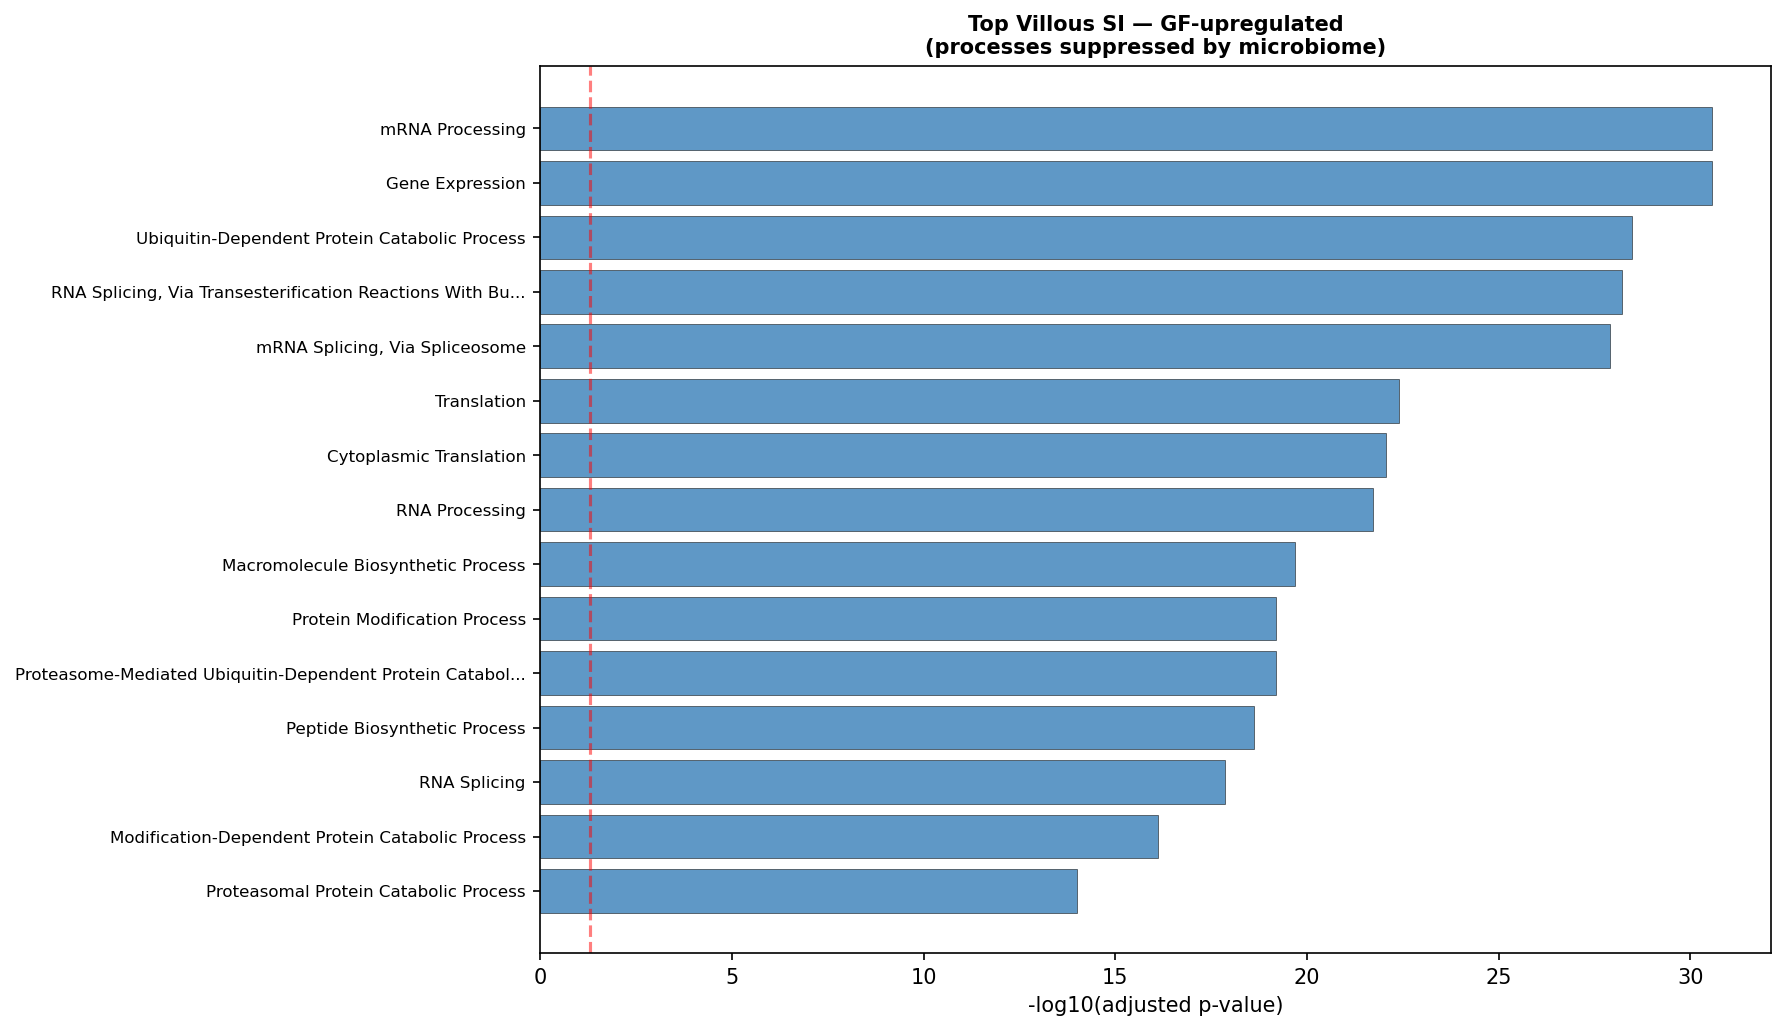
\includegraphics[width=0.6\textwidth]{05_go_top_villous_gf_up.png}
    \caption{GO Biological Process enrichment for genes upregulated 
    at the villus tip in germ-free mice — processes suppressed by 
    the microbiome at the villus tip.}
    \label{fig:go_tip}
\end{figure}

These results indicate that the microbiome suppresses gene expression 
and protein synthesis machinery at the villus tip in normal mice. 
In germ-free mice, this suppression is absent, leading to 
upregulation of transcriptional and translational processes at 
the most exposed epithelial surface.

% =========================================================
\section{Discussion}
% =========================================================

In this study I characterized the transcriptional architecture of 
the small intestinal villus using Visium spatial transcriptomics 
data from Mayassi et al. 2024, extending their analysis from a 
colon-focused perspective to an examination of the 
crypt-to-villus axis across all four SI segments.

My first main finding is that the crypt-to-villus transcriptional 
gradient is organized as a conserved core program shared across 
duodenum, jejunum, and ileum, overlaid with region-specific gene 
expression that increases toward the villus tip. The conserved 
crypt program reflects universal stem cell and proliferation 
machinery — consistent with the known biology of intestinal 
stem cells \cite{gehart2019tales}. The conserved 
tip program reflects the secretory pathway and vesicle transport, consistent 
with the known function of mature enterocytes in secreting 
chylomicrons via the Golgi apparatus \cite{abumrad2012intestinal}. 
The increasing region-specificity toward the villus tip takes place, 
probably, due to the segment-specific functional specializations of mature 
enterocytes — duodenal enterocytes absorb iron and calcium, 
jejunal enterocytes absorb fatty acids and amino acids via 
distinct transporter sets, and ileal enterocytes reabsorb 
bile acids via specific transporters.

My second main finding concerns the microbiome's differential effect 
along the crypt-to-villus axis. I initially hypothesized that the 
villus tip, being directly exposed to the gut lumen, would show the 
greatest microbiome sensitivity. This hypothesis was not confirmed. 
Instead, I found that the bottom villous SI is the most 
microbiome-promoted layer, and — more surprisingly — that the villus 
tip is transcriptionally hyperactive in germ-free mice, with 
upregulation of mRNA processing, translation, and protein catabolism. 
One possible interpretation is that this represents microbiome-induced 
transcriptional suppression at the villus tip, potentially preventing 
excessive inflammatory responses to luminal bacteria. However, 
alternative explanations — such as compensatory upregulation in the 
absence of microbial stimulation, or morphological differences in 
GF villus structure — cannot be excluded with the current data. 
This is consistent with the known role of commensal bacteria in 
maintaining intestinal immune homeostasis \cite{hooper2012interactions}.


\subsection{Limitations}

Several limitations should be noted. First, Visium technology 
captures RNA from multiple cells per spot (~5-15 cells at 
55 $\mu$m resolution), meaning my layer-level analyses reflect 
averaged expression rather than true single-cell resolution. 
Future analyses using single-cell RNA sequencing or higher-resolution 
spatial methods (such as Xenium, which is also available in the 
Mayassi et al. dataset) could provide finer characterization 
of the crypt-to-villus gradient. Second, all data are from 
mouse tissue, and while mouse and human intestinal biology 
are broadly conserved, direct translation to human disease 
requires validation in human samples. Third, the microbiome 
comparison is limited to SPF vs GF; the FMT condition, which 
would allow assessment of microbiome rescue effects, was 
not analyzed due to time constraints. Fourth, the number of 
DEGs detected is influenced by spot count even after 
downsampling, as larger absolute numbers of spots per 
condition increase statistical power for detecting small 
effect sizes. Finally, the villus tip markers identified here could be 
contextualized against published transcriptomic datasets from 
intestinal disease models — such as celiac disease, where 
villous atrophy selectively destroys the tip compartment — 
to directly quantify which conserved tip programs are disrupted 
during pathology.

\subsection{Conclusions}

I have shown that the small intestinal villus is organized 
as a conserved transcriptional gradient shared across all SI 
segments, with region-specific gene expression increasing 
toward the absorptive surface. The microbiome asymmetrically 
affects this gradient, primarily promoting expression in the 
transitional bottom villous zone and suppressing gene 
expression machinery at the villus tip. These findings provide 
a spatially resolved molecular baseline for the small intestinal 
epithelium that could inform future studies of villous atrophy 
in celiac disease and other enteropathies.


\bibliographystyle{unsrtnat}
\bibliography{references}

% =========================================================
\section*{Note on the Use of Large Language Models}
% =========================================================

This project was completed with the assistance of Claude (Anthropic), 
a large language model. It was used to check the correctness of the code,
generation of snakemake file and template for this report.

\end{document}